\documentclass[12pt,]{article}
\usepackage{lmodern}
\usepackage{amssymb,amsmath,stmaryrd}
\usepackage{ifxetex,ifluatex}
\usepackage{fixltx2e} % provides \textsubscript
\ifnum 0\ifxetex 1\fi\ifluatex 1\fi=0 % if pdftex
  \usepackage[T1]{fontenc}
  \usepackage[utf8]{inputenc}
\else % if luatex or xelatex
  \ifxetex
    \usepackage{mathspec}
  \else
    \usepackage{fontspec}
  \fi
  \defaultfontfeatures{Ligatures=TeX,Scale=MatchLowercase}
\fi
% use upquote if available, for straight quotes in verbatim environments
\IfFileExists{upquote.sty}{\usepackage{upquote}}{}
% use microtype if available
\IfFileExists{microtype.sty}{%
\usepackage{microtype}
\UseMicrotypeSet[protrusion]{basicmath} % disable protrusion for tt fonts
}{}
\usepackage[margin=1in]{geometry}
\usepackage{hyperref}
\PassOptionsToPackage{usenames,dvipsnames}{color} % color is loaded by hyperref
\hypersetup{unicode=true,
            pdftitle={Extending ggplot2 for linked and dynamic web graphics},
            pdfkeywords={Animation, Multiple linked views, Statistical graphics, Exploratory data
analysis, Web technologies},
            colorlinks=true,
            linkcolor=cyan,
            citecolor=black,
            urlcolor=Blue,
            breaklinks=true}
\urlstyle{same}  % don't use monospace font for urls
\usepackage{color}
\usepackage{fancyvrb}
\newcommand{\VerbBar}{|}
\newcommand{\VERB}{\Verb[commandchars=\\\{\}]}
\DefineVerbatimEnvironment{Highlighting}{Verbatim}{commandchars=\\\{\}}
% Add ',fontsize=\small' for more characters per line
\usepackage{framed}
\definecolor{shadecolor}{RGB}{248,248,248}
\newenvironment{Shaded}{\begin{snugshade}}{\end{snugshade}}
\newcommand{\AlertTok}[1]{\textcolor[rgb]{0.94,0.16,0.16}{#1}}
\newcommand{\AnnotationTok}[1]{\textcolor[rgb]{0.56,0.35,0.01}{\textbf{\textit{#1}}}}
\newcommand{\AttributeTok}[1]{\textcolor[rgb]{0.77,0.63,0.00}{#1}}
\newcommand{\BaseNTok}[1]{\textcolor[rgb]{0.00,0.00,0.81}{#1}}
\newcommand{\BuiltInTok}[1]{#1}
\newcommand{\CharTok}[1]{\textcolor[rgb]{0.31,0.60,0.02}{#1}}
\newcommand{\CommentTok}[1]{\textcolor[rgb]{0.56,0.35,0.01}{\textit{#1}}}
\newcommand{\CommentVarTok}[1]{\textcolor[rgb]{0.56,0.35,0.01}{\textbf{\textit{#1}}}}
\newcommand{\ConstantTok}[1]{\textcolor[rgb]{0.00,0.00,0.00}{#1}}
\newcommand{\ControlFlowTok}[1]{\textcolor[rgb]{0.13,0.29,0.53}{\textbf{#1}}}
\newcommand{\DataTypeTok}[1]{\textcolor[rgb]{0.13,0.29,0.53}{#1}}
\newcommand{\DecValTok}[1]{\textcolor[rgb]{0.00,0.00,0.81}{#1}}
\newcommand{\DocumentationTok}[1]{\textcolor[rgb]{0.56,0.35,0.01}{\textbf{\textit{#1}}}}
\newcommand{\ErrorTok}[1]{\textcolor[rgb]{0.64,0.00,0.00}{\textbf{#1}}}
\newcommand{\ExtensionTok}[1]{#1}
\newcommand{\FloatTok}[1]{\textcolor[rgb]{0.00,0.00,0.81}{#1}}
\newcommand{\FunctionTok}[1]{\textcolor[rgb]{0.00,0.00,0.00}{#1}}
\newcommand{\ImportTok}[1]{#1}
\newcommand{\InformationTok}[1]{\textcolor[rgb]{0.56,0.35,0.01}{\textbf{\textit{#1}}}}
\newcommand{\KeywordTok}[1]{\textcolor[rgb]{0.13,0.29,0.53}{\textbf{#1}}}
\newcommand{\NormalTok}[1]{#1}
\newcommand{\OperatorTok}[1]{\textcolor[rgb]{0.81,0.36,0.00}{\textbf{#1}}}
\newcommand{\OtherTok}[1]{\textcolor[rgb]{0.56,0.35,0.01}{#1}}
\newcommand{\PreprocessorTok}[1]{\textcolor[rgb]{0.56,0.35,0.01}{\textit{#1}}}
\newcommand{\RegionMarkerTok}[1]{#1}
\newcommand{\SpecialCharTok}[1]{\textcolor[rgb]{0.00,0.00,0.00}{#1}}
\newcommand{\SpecialStringTok}[1]{\textcolor[rgb]{0.31,0.60,0.02}{#1}}
\newcommand{\StringTok}[1]{\textcolor[rgb]{0.31,0.60,0.02}{#1}}
\newcommand{\VariableTok}[1]{\textcolor[rgb]{0.00,0.00,0.00}{#1}}
\newcommand{\VerbatimStringTok}[1]{\textcolor[rgb]{0.31,0.60,0.02}{#1}}
\newcommand{\WarningTok}[1]{\textcolor[rgb]{0.56,0.35,0.01}{\textbf{\textit{#1}}}}
\usepackage{longtable,booktabs}
\usepackage{graphicx,grffile}
\makeatletter
\def\maxwidth{\ifdim\Gin@nat@width>\linewidth\linewidth\else\Gin@nat@width\fi}
\def\maxheight{\ifdim\Gin@nat@height>\textheight\textheight\else\Gin@nat@height\fi}
\makeatother
% Scale images if necessary, so that they will not overflow the page
% margins by default, and it is still possible to overwrite the defaults
% using explicit options in \includegraphics[width, height, ...]{}
\setkeys{Gin}{width=\maxwidth,height=\maxheight,keepaspectratio}
\IfFileExists{parskip.sty}{%
\usepackage{parskip}
}{% else
\setlength{\parindent}{0pt}
\setlength{\parskip}{6pt plus 2pt minus 1pt}
}
\setlength{\emergencystretch}{3em}  % prevent overfull lines
\providecommand{\tightlist}{%
  \setlength{\itemsep}{0pt}\setlength{\parskip}{0pt}}
\setcounter{secnumdepth}{5}
% Redefines (sub)paragraphs to behave more like sections
\ifx\paragraph\undefined\else
\let\oldparagraph\paragraph
\renewcommand{\paragraph}[1]{\oldparagraph{#1}\mbox{}}
\fi
\ifx\subparagraph\undefined\else
\let\oldsubparagraph\subparagraph
\renewcommand{\subparagraph}[1]{\oldsubparagraph{#1}\mbox{}}
\fi

%%% Use protect on footnotes to avoid problems with footnotes in titles
\let\rmarkdownfootnote\footnote%
\def\footnote{\protect\rmarkdownfootnote}

% ------------------------------------------------------------------------------
% Start of JCGS specific titlepage
% ------------------------------------------------------------------------------

\usepackage{tabularx}

\usepackage{amsthm}
\newtheorem{theorem}{Theorem}[section]
\newtheorem{lemma}{Lemma}[section]
\theoremstyle{definition}
\newtheorem{definition}{Definition}[section]
\newtheorem{corollary}{Corollary}[section]
\newtheorem{proposition}{Proposition}[section]
\theoremstyle{definition}
\newtheorem{example}{Example}[section]
\theoremstyle{definition}
\newtheorem{exercise}{Exercise}[section]
\theoremstyle{remark}
\newtheorem*{remark}{Remark}
\newtheorem*{solution}{Solution}
\begin{document}

\def\spacingset#1{\renewcommand{\baselinestretch}%
{#1}\small\normalsize} \spacingset{1}

\title{\bf Extending ggplot2 for linked and dynamic web graphics}
\author{
  Carson Sievert \\ 
  Department of Statistics, Iowa State University \\
  Susan VanderPlas \\
  Department of Statistics, Iowa State University \\
  Jun Cai \\
  Department of Earth System Science, Tsinghua University\\
  Kevin Ferris \\
  Baseball Operations Department, Tampa Bay Rays \\
  Faizan Uddin Fahad Khan \\
  Department of Computer Science \& Engineering, IIT BHU \\
  Toby Dylan Hocking \\ 
  Department of Human Genetics, McGill University \\
}
\maketitle

\bigskip
\begin{abstract}
% 200 or fewer words
Interactive web graphics are great for communication and knowledge
sharing, but are difficult to leverage during the exploratory phase of a
data science workflow. Even before the web, interactive graphics helped
data analysts quickly gather insight from data, discover the unexpected,
and develop better model diagnostics. Web technologies, however, are not
designed to fit inside an exploratory data analysis workflow where rapid
iteration between data manipulation, modeling, and visualization must
occur. We propose the R package \textbf{animint} for rapid creation of
linked and animated web graphics through a simple extension of
\textbf{ggplot2}'s implementation of the Grammar of Graphics. The
extension allows users to use their existing \textbf{ggplot2} code, then
leverage an idomatic API for describing animations and graphical queries
between multiple linked views.
\end{abstract}

\noindent
{\it Keywords:}  Animation, Multiple linked views, Statistical graphics, Exploratory data
analysis, Web technologies
\vfill

\newpage
\spacingset{1.45} % DON'T change the spacing!

% ------------------------------------------------------------------------------
% End of JCGS specific titlepage
% ------------------------------------------------------------------------------

\hypertarget{intro}{%
\section{Introduction}\label{intro}}

For more than a half century now, statisticians have designed, built,
and used interactive graphics for exploring high-dimensional data and
better informing their modeling process. In fact, the ASA maintains a
video library (\url{http://stat-graphics.org/movies/}) to document and
demonstrate applications of instrumental interactive statistical
graphics systems such as \texttt{PRIM-9} (Fisherkeller and Tukey 1988),
\texttt{Dataviewer} (Andreas Buja and McDonald 1988), \texttt{XGobi}
(Swayne and Buja 1998), \texttt{GGobi} (D. Cook and Swayne 2007), and
\texttt{Mondrian} (Theus 2002). These, as well as other influential
systems, such as \texttt{LISP-STAT} (Tierney 1990) and \texttt{MANET}
(Unwin A. 1996), all have a rich support for accomplishing a wide
variety of statistical analysis tasks, and most were developed before
the web browser had rich graphics support.

All of these systems, as well as some more modern systems, such as
\textbf{rggobi} (Duncan Temple Lang 2016), \textbf{iplots} (Urbanek
2011), \textbf{loon} (Waddell and Oldford 2018), etc, require a heavy
set of computational dependencies in order to view or interact with
graphics. Although this allows the freedom to easily leverage libraries
with sophicated statistical functionality, it limits the ability to
share or embed such graphics in a larger document. On the other hand,
interactive web graphics are now ubiquitous because of their
accessibility and composability.

Generally speaking, web graphics that use purely ``client-side''
technologies (i.e., \texttt{HTML}, \texttt{SVG}, \texttt{CSS}, and
\texttt{JavaScript}) are desired for their sharability, scalabaility,
and maintainability. This is why many web-based graphing libraries work
entirely with client-side technologies, like Vega (Trifacta 2014),
plotly.js, and bokeh.\\
Unfortunately, client-side technologies are not particularly well-suited
for statistical computation, which we often want to leverage via dynamic
controls in an interactive statistical graphics system; but when
necessary, one can leverage a client-server model.

Table X gives a high-level depiction of the different infrastructure
required for a purely client-side (i.e.~standalone) webpage versus a
client-server web application. Focusing just on the R language, there
are now a number of ways to develop web applications powered by R,
including \textbf{FastRWeb} (Urbanek and Horner 2015), \textbf{opencpu}
(Ooms 2014), and \textbf{plumber} (Trestle Technology, LLC 2017), but
\textbf{shiny} (RStudio 2013) is most widely used since it provides a
nice reactive programming framework in addition to client-server
communication.

\begin{itemize}
\tightlist
\item
  Make an argument that we need more R -\textgreater{} HTML interfaces
  that don't require a callback to R.
\end{itemize}

D. Cook, Buja, and Swayne (2007) taxonomy motivated by data analysis
tasks

Interactive graphics are an important part of applied statistical
practice, because they can lead to a better understanding of
high-dimensional data sets and models. Interactive graphics are useful
in the context of EDA, model selection/validation, and presenting
results of an analysis. Interactive graphics toolkits in R have been
available for decades, but these approaches are often not easy to
reproduce or distribute to a larger audience. It is true that most
graphics generated during EDA are ultimately not useful, but sometimes,
understanding gained during this phase is most easily shared via the
interactive graphics themselves. Thus, there is value in being able to
easily share and embed interactive graphics inside a larger report.
Unfortunately, this is typically hard, if not impossible, using
traditional interactive graphics toolkits. As a result, there is a large
disconnect between the visualization tools that we use for exploration
versus presentation.

One of the most widely used R packages is \textbf{ggplot2} (Wickham
2009), a data visualization package inspired by the grammar of graphics
(Wilkinson et al. 2006). In fact, Donoho (2015) writes: ``This effort
may have more impact on today's practice of data analysis than many
highly-regarded theoretical statistics papers''. In our experience,
\textbf{ggplot2} has made an impact thanks to its foundation in the
grammar of graphics, carefully chosen defaults, and overall usability.
This helps data analysts rapidly iterate and discover informative
visualizations -- an essential task in exploratory data analysis (EDA).
When dealing with high-dimensional data, however, it is often useful to
produce interactive and/or dynamic graphics, which \textbf{ggplot2} does
not inherently support.

We aim to narrow this gap in visualization tools by extending
\textbf{ggplot2}'s grammar of graphics implementation for interactive
and dynamic web graphics. Our extension allows one to create animated
transitions and perform dynamic queries via direct manipulation of
linked views like those described in Ahlberg, Williamson, and
Shneiderman (1991) and Buja et al. (1991). A conceptual model for our
extension is provided in Section \ref{extension} and Section
\ref{animation}. In Section \ref{worldbank}, we demonstrate our
extension with an example. In Section \ref{implementation}, we outline
design decisions made in our implementation in the R package
\textbf{animint}. In Section \ref{performance}, we provide a sense of
the scope of our system and its performance limitations through a
handful of examples. In Section \ref{compare}, we conduct a comparison
study by replicating examples with other leading systems. Finally, in
Section \ref{limitations}, we discuss future work and limitations of our
current system.

\hypertarget{related-work}{%
\section{Related work}\label{related-work}}

We aim to provide a system which empowers \textbf{ggplot2} users to go
beyond the confines of static graphics with minimal friction imposed
upon their current workflow. We acknowledge that numerous systems which
support similar visualization techniques exist outside of the R
ecosystem, but we intentionally focus on R interfaces since the
surrounding statistical computing environment is crucial for enabling an
efficient EDA workflow.

It is important to acknowledge that \textbf{ggplot2} is built on top of
the R package \textbf{grid}, a low-level graphics system, which is now
bundled with R itself (R Core Team 2017). Neither \textbf{grid}, nor
\textbf{base} R graphics, have strong support for handling user
interaction, which creates a need for add-on packages. There are a
number of approaches these packages take to rendering, each with their
own benefits and drawbacks. Traditionally, they build on low-level R
interfaces to graphical systems such as GTK+ (Lawrence and Temple Lang
2010), Qt (Lawrence and Sarkar 2016), or Java GUI frameworks (Urbanek
2016). In general, the resulting system can be very fast and flexible,
but sharing and reproducing output is usually a problem due to the heavy
software requirements. Although there may be sacrifices in performance,
using the modern web browser as a canvas is more portable, accessible,
and composable (graphics can be embedded within larger
frameworks/documents).

Base R does provide a Scalable Vector Graphics (SVG) device,
\texttt{svg()}, via the Cairo graphics API (Cairo 2016). The R package
\textbf{SVGAnnotation} provides functionality to post-process
\texttt{svg()} output in order to add interactive and dynamic features
(Nolan and Lang 2012). This is a powerful approach, since in theory it
can work with any R graphic, but the package is self-described as a
proof-of-concept which reverse-engineers poorly-structured
\texttt{svg()} output. As a result, it is not straightforward to extend
this system for linked data visualizations with advanced functionality
(multiple layers, multiple plots, multiple selection variables).

The lack of well-structured SVG for R graphics motivated the
\textbf{gridSVG} package which provides sensible structuring of SVG
output for grid graphics (Murrell and Potter 2015). This package also
provides some low-level tools for animating or adding interactive
features, where grid objects must be referenced by name. As a result,
use of this interface to add interactivity to a \textbf{ggplot2} plot
requires understanding of the grid naming scheme \textbf{ggplot2} uses
internally. An interface where interactivity can be expressed by
referencing the data to be visualized, rather than the building blocks
of the graphics system, would be preferable since the former interface
is decoupled from the implementation and does not require knowledge of
grid.

In terms of the animation API, the R package \textbf{gganimate} is very
similar to our system (Robinson 2016). It directly extends
\textbf{ggplot2} by adding a new aesthetic, named \texttt{frame}, which
splits the data into subsets (one for each unique value of the frame
variable), produces a static plot for each subset, and uses the
animation package to combine the images into a key frame animation (Xie
2013). This is quite similar but not as flexible as our system's support
for animation, which we fully describe in Section \ref{animation}.
Either system has the ability to control the amount of time that a given
frame is displayed, but our system can also animate the transition
between frames via the \texttt{d3.transition()} API (Bostock,
Oglevetsky, and Heer 2011). Smooth transitions help the animation viewer
track positions between frames, which is useful in many scenarios, such
as the touring example discussed in Section \ref{tour}. The
\textbf{tweenr} package provides similar smooth transitions, by
computing data values in R that interpolate between animation frames (in
\textbf{animint}, these calculations are performed in the web browser).

The \textbf{ggvis} package is similar to our system in that is is also
inspired by the grammar of graphics (Chang and Wickham 2015). It does
not directly extend \textbf{ggplot2}, but instead provides a brand new
purely functional interface which is designed with interactive graphics
in mind. It currently relies on Vega to render the SVG graphics from
JSON (Trifacta 2014), and the R package \textbf{shiny} to enable many of
its interactive capabilities (RStudio 2013). The interface gives
tremendous power to R users, as it allows one to write R functions to
handle user events. This power does come with a cost, though, as sharing
and hosting ggvis graphics typically requires special web server
softwares, even when the interaction logic could be handled entirely
client-side. As we outline in Section \ref{implementation}, our system
does not require a web server, but can also be used inside
\textbf{shiny} web applications, when desired.

The tour is a useful visualization technique for exploring
high-dimensional data which requires interactive and dynamic graphics.
The open-source software ggobi is currently the most fully-featured
toolkit for touring data and has support for interactive techniques such
as linking, zooming, panning, and identifying (D. Cook and Swayne 2007).
The R package \textbf{rggobi} (Duncan Temple Lang 2016) provides an R
interface to ggobi's graphical interface, but unfortunately, the
software requirements for installation and use of this toolchain are
heavy and stringent. Furthermore, sharing the interactive versions of
these graphics are not possible. The R package \textbf{cranvas} aims to
be the successor to ggobi, with support for similar interactive
techniques, but with a more flexible interface for describing plots
inspired by the grammar of graphics (Xie et al. 2013). \textbf{Cranvas}
also has heavy and stringent software requirements which limits the
portability and accessibility of the software.

Another R package for interactive graphics is \textbf{iplots} (Urbanek
2011), which has several important differences compared to
\textbf{animint}. Brushing/highlighting of linked iplots is supported
for single-layer plots such as scatterplots or barplots, but it is not
easy to define new multi-layer interactive plots. Futhermore since
iplots does not use the grammar of graphics, it is difficult to create
legends and multi-panel plots. Finally since iplots requires compiled
C++ code for rendering on the local machine, its graphics are not as
easy to share as \textbf{animint} graphics which can be viewed in a web
browser.

\hypertarget{extending-the-layered-grammar-of-graphics}{%
\section{Extending the layered grammar of
graphics}\label{extending-the-layered-grammar-of-graphics}}

\begin{table}

\caption{
New features that animint adds to the grammar of graphics.
}\label{tab:overview}
\small
\begin{tabularx}{\textwidth}{rl}
Feature & Description \\
\hline
clickSelects & aesthetic for a geom which can be clicked to update the current selection.  \\
showSelected & aesthetic for a geom which plots only the data corresponding to the current selection.  \\
selector.types & global option to specify single or multiple selection for each interaction variable.  \\
first & global option to specify first selection.  \\
time & global option to specify delay between animation frames.  \\
duration & global option to specify smooth transitions.  \\
key & aesthetic specifying variable to use for matching data in smooth transitions. \\
\hline
\end{tabularx}

\end{table}

In this section, we propose several extensions to the layered grammar of
graphics (Table\textasciitilde{}\ref{tab:overview}). Our extensions
enable declarative expression of animations and dynamic queries via
direct manipulation. In \textbf{ggplot2}, there are five essential
components that define a layer of graphical makings: data, mappings
(i.e., aesthetics), geometry, statistic, and position. These simple
components are easily understood in isolation and can be combined in
many ways to express a wide array of graphics. For a simple example,
here is one way to create a scatterplot in \textbf{ggplot2} of variables
named \texttt{\textless{}X\textgreater{}} and
\texttt{\textless{}Y\textgreater{}} in
\texttt{\textless{}DATA\textgreater{}}:

\begin{Shaded}
\begin{Highlighting}[]
\KeywordTok{ggplot}\NormalTok{() }\OperatorTok{+}\StringTok{ }\KeywordTok{layer}\NormalTok{(}
  \DataTypeTok{data =} \OperatorTok{<}\NormalTok{DATA}\OperatorTok{>}\NormalTok{, }
  \DataTypeTok{mapping =} \KeywordTok{aes}\NormalTok{(}\DataTypeTok{x =} \OperatorTok{<}\NormalTok{X}\OperatorTok{>}\NormalTok{, }\DataTypeTok{y =} \OperatorTok{<}\NormalTok{Y}\OperatorTok{>}\NormalTok{), }
  \DataTypeTok{geom =} \StringTok{"point"}\NormalTok{, }
  \DataTypeTok{stat =} \StringTok{"identity"}\NormalTok{,}
  \DataTypeTok{position =} \StringTok{"identity"}
\NormalTok{)}
\end{Highlighting}
\end{Shaded}

For every geometry, \textbf{ggplot2} provides a convenient wrapper
around \texttt{layer()} which provides sensible defaults for the
statistic and position (in this case, both are ``identity''):

\begin{Shaded}
\begin{Highlighting}[]
\KeywordTok{ggplot}\NormalTok{() }\OperatorTok{+}\StringTok{ }\KeywordTok{geom_point}\NormalTok{(}
  \DataTypeTok{data =} \OperatorTok{<}\NormalTok{DATA}\OperatorTok{>}\NormalTok{, }
  \KeywordTok{aes}\NormalTok{(}\DataTypeTok{x =} \OperatorTok{<}\NormalTok{X}\OperatorTok{>}\NormalTok{, }\DataTypeTok{y =} \OperatorTok{<}\NormalTok{Y}\OperatorTok{>}\NormalTok{)}
\NormalTok{)}
\end{Highlighting}
\end{Shaded}

A single \textbf{ggplot2} plot can be comprised of multiple layers, and
different layers can correspond to different data. Since each graphical
mark within a \textbf{ggplot2} layer corresponds to one (or more)
observations in \texttt{\textless{}DATA\textgreater{}}, aesthetic
mappings provide a mechanism for mapping graphical selections to the
original data (and vice-versa) which is essential to any interactive
graphics system (Wickham et al. 2010). Thus, given a way to combine
multiple \textbf{ggplot2} plots into a single view, this design can be
extended to support a notion of multiple linked views, as those
discussed in Ahlberg, Williamson, and Shneiderman (1991) and Buja et al.
(1991).

\hypertarget{extension}{%
\subsection{Direct manipulation of dynamic queries}\label{extension}}

Direct manipulation, as discussed in Ahlberg, Williamson, and
Shneiderman (1991), is a graphical interface for interacting with
databases. Direct manipulation interfaces include a graphical
representation of queries to the database, which can be manipulated
using the mouse. In the context of statistical graphics, direct
manipulation refers to interfaces in which clicking the plotted
representation of the data (such as lines or points) changes the plot.
In contrast, indirect manipulation interfaces use widgets (such as
buttons or menus) to change the plot.

D. Cook and Swayne (2007) use SQL queries to formalize the direct
manipulation methods discussed in Ahlberg, Williamson, and Shneiderman
(1991) and Buja et al. (1991). We propose to embed this direct
manipulation framework inside the layered grammar of graphics with two
new aesthetics, \texttt{clickSelects} and \texttt{showSelected}.

\begin{itemize}
\tightlist
\item
  \texttt{clickSelects} defines a selection source via a mouse click.
  For example \texttt{aes(clickSelects=year)} designates a plot element
  which, when clicked, will change the selected value of the
  \texttt{year} variable.
\item
  \texttt{showSelected} defines a selection target. For example
  \texttt{aes(showSelected=year)} means to only show a plot element for
  data with the currently selected value of the \texttt{year} variable.
\end{itemize}

Below, we use \textbf{animint} to create a linked view between a bar
chart and a scatter plot, where the user can click on bars to control
the points shown in the scatterplot. This is shown in the video in
Figure \ref{fig:tips}. As a result, we can quickly see how the
relationship among tip amount and total bill amount depends on whether
the customer is smoker.

\begin{Shaded}
\begin{Highlighting}[]
\NormalTok{gg.bar <-}\StringTok{ }\KeywordTok{ggplot}\NormalTok{() }\OperatorTok{+}\StringTok{ }\KeywordTok{geom_bar}\NormalTok{(}
  \DataTypeTok{data =}\NormalTok{ reshape2}\OperatorTok{::}\NormalTok{tips, }
  \KeywordTok{aes}\NormalTok{(}\DataTypeTok{x =}\NormalTok{ smoker, }\DataTypeTok{clickSelects =}\NormalTok{ smoker)}
\NormalTok{)}
\NormalTok{gg.scatter <-}\StringTok{ }\KeywordTok{ggplot}\NormalTok{() }\OperatorTok{+}\StringTok{ }\KeywordTok{geom_point}\NormalTok{(}
  \DataTypeTok{data =}\NormalTok{ reshape2}\OperatorTok{::}\NormalTok{tips, }
  \KeywordTok{aes}\NormalTok{(}\DataTypeTok{x =}\NormalTok{ total_bill, }\DataTypeTok{y =}\NormalTok{ tip, }
      \DataTypeTok{showSelected =}\NormalTok{ smoker)}
\NormalTok{)}
\end{Highlighting}
\end{Shaded}

\begin{figure}
\centering
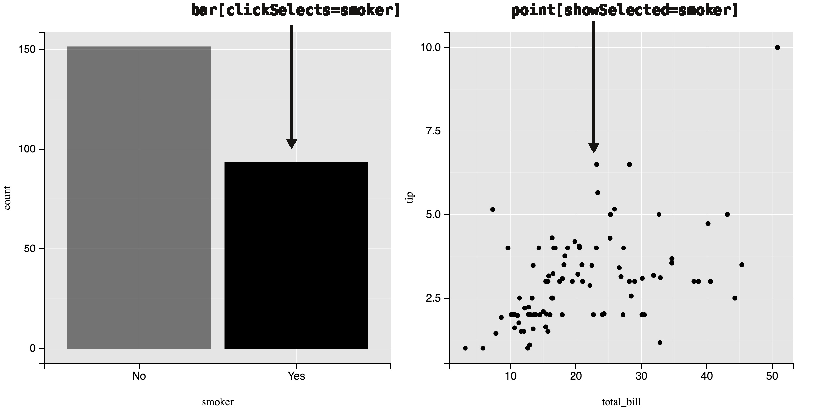
\includegraphics{images/figure-tips}
\caption{\label{fig:tips}Linked dynamic querying via direct manipulation
using animint. The \texttt{clickSelects} aesthetic designates a
clickable geom that can change a selection variable, and the
\texttt{showSelected} aesthetic designates a geom that responds by
showing only the data which corresponds to the current selection. A
video demonstration can be viewed online at
\url{https://vimeo.com/160496419}}
\end{figure}

In the R code above, the proposed \texttt{showSelected} and
\texttt{clickSelects} aesthetics are used to link the two ggplots, since
they refer to a common variable, \texttt{smoker}. Each variable that is
used in a \texttt{clickSelects} or \texttt{showSelected} aesthetic is
treated as a selection variable with an interactively updated set of
selected values that is used to dynamically update the plots in response
to user input. In the first plot above, we have used
\texttt{aes(clickSelects=smoker)} to specify a bar with direct
manipulation (mouse clicks on the barplot) that dynamically changes the
\texttt{smoker} selection variable. In the second plot above, we have
used \texttt{aes(showSelected=smoker)} to specify that we only want to
show data points for the current selection of the \texttt{smoker}
variable. In response to a user clicking on the bars in the first plot,
our system essentially performs the SQL query below in order to generate
the data to display in the second plot:

\begin{Shaded}
\begin{Highlighting}[]
\KeywordTok{SELECT}\NormalTok{ * }\KeywordTok{FROM}\NormalTok{ tips}
  \KeywordTok{WHERE}\NormalTok{ smoker }\KeywordTok{IN}\NormalTok{ smoker_selection}
\end{Highlighting}
\end{Shaded}

In this example, \texttt{smoker\_selection} is either ``Yes'' or ``No''
(a single selected value), but as we show in later examples,
\texttt{smoker\_selection} can also be an array of values (multiple
selected values). Although the \texttt{clickSelects} aesthetic is tied
to a mouse click event, other aesthetics could easily be created to
support other selection events, such as hover or click+drag.
Statistically speaking, this type of visualization is useful for
navigating through joint distributions conditional upon discrete values.
In this sense, our extension is closely related to trellis displays
(Becker, Cleveland, and Shyu 2010) and linked scatterplot brushing
(Becker and Cleveland 1987). The major differences are that our
conditioning is layer-specific (not plot-specific), is not tied to a
particular geometry, and can be controlled through direct manipulation
or animation controls.

\hypertarget{worldbank}{%
\subsection{World Bank example}\label{worldbank}}

Figure \ref{fig:worldbank} shows an interactive animation of the World
Bank data set created with our \textbf{animint} implementation (World
Bank 2012). The visualization helps us explore the change in the
relationship between life expectancy and fertility over time for 205
countries. By default, the year 1979 and the countries United States and
Vietnam are selected, but readers are encouraged to watch the video of
the animation and/or interact the visualization using a web
browser.\footnote{\url{http://bl.ocks.org/tdhock/raw/8ce47eebb3039263878f/}}
In the interactive version, the selected value of the year variable is
automatically incremented every few seconds, using animation to
visualize yearly changes in the relationship between life expectancy and
fertility rate.

\begin{figure}
\centering
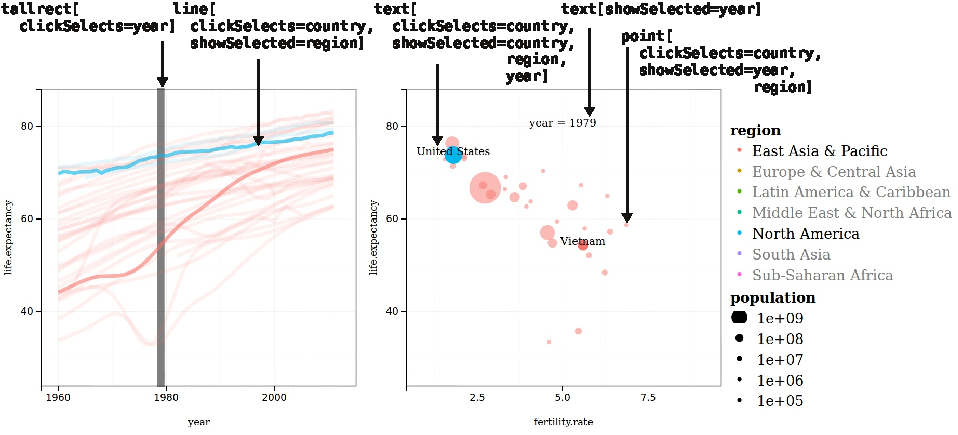
\includegraphics{images/figure-1}
\caption{\label{fig:worldbank}An interactive animation of World Bank
demographic data of several countries, designed using
\texttt{clickSelects} and \texttt{showSelected} keywords (top). Left: a
multiple time series from 1960 to 2010 of life expectancy, with bold
lines showing the selected countries and a vertical grey tallrect
showing the selected year. Right: a scatterplot of life expectancy
versus fertility rate of all countries. The legend and text elements
show the current selection: year=1979, country=\{United States,
Vietnam\}, and region=\{East Asia \& Pacific, North America\}}
\end{figure}

We anticipate that some \textbf{ggplot2} users will be able to reverse
engineer the \textbf{animint} code which creates Figure
\ref{fig:worldbank}, simply by looking at it. In fact, this is a big
reason why \textbf{ggplot2} is so widely used: it helps minimize the
amount of time required to translate an idea for a figure into computer
code. Note that, in the left hand plot of Figure \ref{fig:worldbank}, we
have a time series of the life expectancy where each line is a country
(i.e., we \texttt{group} by country) and lines are colored by region. By
clicking on a line, we also want the country label to appear in the
right hand plot, so we also need to set \texttt{clickSelects=country}.
Lastly, by setting \texttt{showSelected=region}, we can hide/show lines
by clicking on the color legend entries.

\begin{Shaded}
\begin{Highlighting}[]
\NormalTok{timeSeries <-}\StringTok{ }\KeywordTok{ggplot}\NormalTok{() }\OperatorTok{+}\StringTok{ }\KeywordTok{geom_line}\NormalTok{(}
  \DataTypeTok{data =}\NormalTok{ WorldBank,}
  \KeywordTok{aes}\NormalTok{(}\DataTypeTok{x =}\NormalTok{ year, }\DataTypeTok{y =}\NormalTok{ life.expectancy,}
      \DataTypeTok{group =}\NormalTok{ country, }\DataTypeTok{color =}\NormalTok{ region,}
      \DataTypeTok{clickSelects =}\NormalTok{ country, }
      \DataTypeTok{showSelected =}\NormalTok{ region)}
\NormalTok{)}
\end{Highlighting}
\end{Shaded}

We want to provide a visual cue for the selected year in the time
series, so in the code below we add some tall rectangles to the time
series plot. These tall rectangles will also serve as a way to directly
modify the selected year. The tallrect geometry is a special case of a
rectangle that automatically spans the entire vertical range, so we just
have to specify the horizontal range via \texttt{xmin} and \texttt{xmax}
aesthetics. Also, since the layered grammar of graphics allows for
different data in each layer, we supply a data frame with just the
unique years in the entire data for this layer.

\begin{Shaded}
\begin{Highlighting}[]
\NormalTok{years <-}\StringTok{ }\KeywordTok{data.frame}\NormalTok{(}\DataTypeTok{year =} \KeywordTok{unique}\NormalTok{(WorldBank}\OperatorTok{$}\NormalTok{year))}
\NormalTok{timeSeries <-}\StringTok{ }\NormalTok{timeSeries }\OperatorTok{+}\StringTok{ }\KeywordTok{geom_tallrect}\NormalTok{(}
  \DataTypeTok{data =}\NormalTok{ years,}
  \KeywordTok{aes}\NormalTok{(}\DataTypeTok{xmin =}\NormalTok{ year }\OperatorTok{-}\StringTok{ }\FloatTok{0.5}\NormalTok{, }\DataTypeTok{xmax =}\NormalTok{ year }\OperatorTok{+}\StringTok{ }\FloatTok{0.5}\NormalTok{,}
      \DataTypeTok{clickSelects =}\NormalTok{ year)}
\NormalTok{)}
\end{Highlighting}
\end{Shaded}

As for the right hand plot in Figure \ref{fig:worldbank}, there are
three layers: a point layer for countries, a text layer for countries,
and a text layer to display the selected year. By clicking on a point,
we want to display the country text label and highlight the
corresponding time series on the left hand plot, so we set
\texttt{clickSelects=country} in this layer. Furthermore, we only want
to show the points for the selected year and region, so we also need
\texttt{showSelected=year} and \texttt{showSelected2=region}.

\begin{Shaded}
\begin{Highlighting}[]
\NormalTok{scatterPlot <-}\StringTok{ }\KeywordTok{ggplot}\NormalTok{() }\OperatorTok{+}\StringTok{ }\KeywordTok{geom_point}\NormalTok{(}
  \DataTypeTok{data =}\NormalTok{ WorldBank,}
  \KeywordTok{aes}\NormalTok{(}\DataTypeTok{x =}\NormalTok{ fertility.rate, }\DataTypeTok{y =}\NormalTok{ life.expectancy,}
      \DataTypeTok{color =}\NormalTok{ region, }\DataTypeTok{size =}\NormalTok{ population,}
      \DataTypeTok{clickSelects =}\NormalTok{ country,}
      \DataTypeTok{showSelected =}\NormalTok{ year,}
      \DataTypeTok{showSelected2 =}\NormalTok{ region)}
\NormalTok{)}
\end{Highlighting}
\end{Shaded}

Note that any aesthetics containing the substring \texttt{showSelected}
(including \texttt{showSelected2}) are interpreted as
\texttt{showSelected} variables, and combined together using the
intersection operation. In the example above, that means that a point
will be drawn for the currently selected combination of year and region,
as in the following SQL query,

\begin{Shaded}
\begin{Highlighting}[]
\KeywordTok{SELECT}\NormalTok{ * }\KeywordTok{FROM}\NormalTok{ WorldBank}
  \KeywordTok{WHERE} \DataTypeTok{year}   \KeywordTok{IN}\NormalTok{ year_selection}
  \KeywordTok{AND}\NormalTok{   region }\KeywordTok{IN}\NormalTok{ region_selection}
\end{Highlighting}
\end{Shaded}

Below, the text layer for annotating selected countries is essentially
the same as the point layer, except we map the country name to the
\texttt{label} aesthetic.

\begin{Shaded}
\begin{Highlighting}[]
\NormalTok{scatterPlot <-}\StringTok{ }\NormalTok{scatterPlot }\OperatorTok{+}\StringTok{ }\KeywordTok{geom_text}\NormalTok{(}
  \DataTypeTok{data =}\NormalTok{ WorldBank,}
  \KeywordTok{aes}\NormalTok{(}\DataTypeTok{x =}\NormalTok{ fertility.rate, }\DataTypeTok{y =}\NormalTok{ life.expectancy,}
      \DataTypeTok{label =}\NormalTok{ country,}
      \DataTypeTok{showSelected =}\NormalTok{ country,}
      \DataTypeTok{showSelected2 =}\NormalTok{ year,}
      \DataTypeTok{showSelected3 =}\NormalTok{ region)}
\NormalTok{)}
\end{Highlighting}
\end{Shaded}

Lastly, to help identify the selected year when viewing the scatterplot,
we add another layer of text at a fixed location.

\begin{Shaded}
\begin{Highlighting}[]
\NormalTok{scatterPlot <-}\StringTok{ }\NormalTok{scatterPlot }\OperatorTok{+}\StringTok{ }\KeywordTok{geom_text}\NormalTok{(}
  \DataTypeTok{data =}\NormalTok{ years, }\DataTypeTok{x =} \DecValTok{5}\NormalTok{, }\DataTypeTok{y =} \DecValTok{80}\NormalTok{,}
  \KeywordTok{aes}\NormalTok{(}\DataTypeTok{label =} \KeywordTok{paste}\NormalTok{(}\StringTok{"year ="}\NormalTok{, year),}
      \DataTypeTok{showSelected =}\NormalTok{ year)}
\NormalTok{)}
\end{Highlighting}
\end{Shaded}

\hypertarget{animation}{%
\subsection{Linking, animation and other options}\label{animation}}

Linking is declared by putting ggplots with common \texttt{clickSelects}
and \texttt{showSelected} aesthetics together in a list. For example, we
can link the ggplots from the previous section by including them
together as the first two elements of the following list:

\begin{Shaded}
\begin{Highlighting}[]
\NormalTok{viz <-}\StringTok{ }\KeywordTok{list}\NormalTok{(}
  \DataTypeTok{timeSeries =}\NormalTok{ timeSeries,}
  \DataTypeTok{scatterPlot =}\NormalTok{ scatterPlot}
\NormalTok{  )}
\end{Highlighting}
\end{Shaded}

Note that the animint \texttt{viz} list above can also contain rendering
options, as we discuss below (see Table\textasciitilde{}1 for a summary
of new interactive features in \textbf{animint}). For example, the
\texttt{selector.types} option controls whether or not selections for a
given variable can accumulate (single or multiple selected values).

\begin{Shaded}
\begin{Highlighting}[]
\NormalTok{viz}\OperatorTok{$}\NormalTok{selector.types =}\StringTok{ }\KeywordTok{list}\NormalTok{(}
  \DataTypeTok{year =} \StringTok{"single"}\NormalTok{,}
  \DataTypeTok{country =} \StringTok{"multiple"}\NormalTok{,}
  \DataTypeTok{region =} \StringTok{"multiple"}
\NormalTok{  )}
\end{Highlighting}
\end{Shaded}

The code above declares \texttt{year} as a single selection variable,
which means that only a single year may be selected at a time (clicking
a geom with \texttt{clickSelects=year} will change the selection to the
corresponding year). The \texttt{country} and \texttt{region} variables
are declared as multiple selection variables, which can have multiple
selected values at a time (clicking a geom with
\texttt{clickSelects=country} will add/remove that country to/from the
selection set).

Another example is the \texttt{first} option, which controls selected
values when the visualization is first rendered. The code below declares
that the first selection of the \texttt{country} variable is the set of
two countries, United States and Vietnam.

\begin{Shaded}
\begin{Highlighting}[]
\NormalTok{viz}\OperatorTok{$}\NormalTok{first =}\StringTok{ }\KeywordTok{list}\NormalTok{(}\DataTypeTok{country =} \KeywordTok{c}\NormalTok{(}\StringTok{"United States"}\NormalTok{, }\StringTok{"Vietnam"}\NormalTok{))}
\end{Highlighting}
\end{Shaded}

Animation is declared using the \texttt{time} option, which specifies a
selection variable which will be automatically updated over time, as
well as a time delay in milliseconds. The code below declares the
\texttt{year} variable to be animated every 3 seconds.

\begin{Shaded}
\begin{Highlighting}[]
\NormalTok{viz}\OperatorTok{$}\NormalTok{time <-}\StringTok{ }\KeywordTok{list}\NormalTok{(}\DataTypeTok{variable =} \StringTok{"year"}\NormalTok{, }\DataTypeTok{ms =} \DecValTok{3000}\NormalTok{)}
\end{Highlighting}
\end{Shaded}

Animation is useful in the World Bank data visualization because it
shows how the bivariate relationship between fertility rate and life
expectancy changes over time. Animation clearly shows how many countries
progress from low life expectancy and high fertility rate in early
years, to high life expectancy and low fertility rate in later years.

Finally, the \texttt{duration} option specifies the amount of time used
to smoothly transition between selections (with linear easing). Smooth
transitions help the viewer track geoms before and after an update to
the selection set. For example in the code below we declare a 1 second
smooth transition on the \texttt{year} variable, in order to more easily
track the points on the scatterplot.

\begin{Shaded}
\begin{Highlighting}[]
\NormalTok{viz}\OperatorTok{$}\NormalTok{duration <-}\StringTok{ }\KeywordTok{list}\NormalTok{(}\DataTypeTok{year =} \DecValTok{1000}\NormalTok{)}
\end{Highlighting}
\end{Shaded}

Note that for accurate interpretation of smooth transitions, the new
\texttt{key} aesthetic must be specified. The \texttt{key} aesthetic is
used to match data elements before and after the smooth transition. In
the World Bank example, we would need to specify
\texttt{aes(key=country)} for the points and text in the scatterplot.

\hypertarget{compiling-and-rendering}{%
\subsection{Compiling and rendering}\label{compiling-and-rendering}}

\begin{figure}
\centering
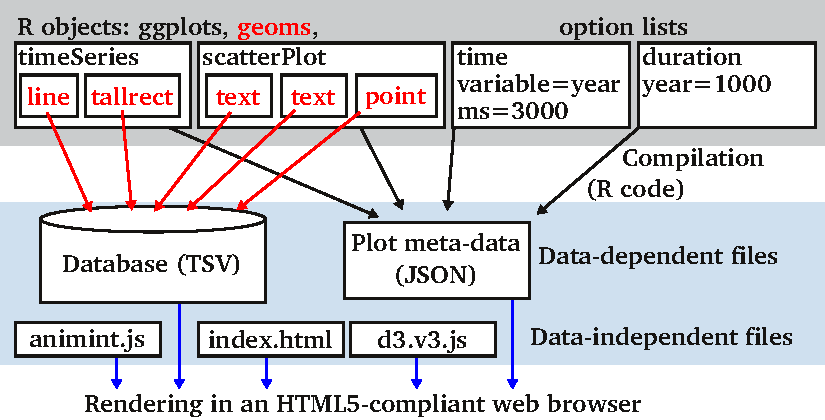
\includegraphics{images/figure-design.pdf}
\caption{\label{fig:design}A schematic explanation of compilation and
rendering in the World Bank visualization. Top: the interactive
animation is a list of 4 R objects: 2 ggplots and 2 option lists.
Center: \textbf{animint} R code compiles data in ggplot geoms to a
database of TSV files (\textcolor{red}{$\rightarrowtriangle$}). It also
compiles plot meta-data including ggplot aesthetics, animation time
options, and transition duration options to a JSON meta-data file
(\(\rightarrowtriangle\)). Bottom: those data-dependent compiled files
are combined with data-independent JavaScript and HTML files which
render the interactive animation in a web browser
(\textcolor{blue}{$\rightarrowtriangle$}).}
\end{figure}

Supplying the \texttt{viz} list of ggplots and rendering options to the
\texttt{animint2dir()} function will save all the files necessary for
rendering the visualization:

\begin{Shaded}
\begin{Highlighting}[]
\KeywordTok{animint2dir}\NormalTok{(viz)}
\end{Highlighting}
\end{Shaded}

As shown in Figure \ref{fig:design}, the \textbf{animint} system is
implemented in 2 parts: the compiler and the renderer. The compiler is
implemented in R code that converts a list of ggplots and options to a
JSON plot meta-data file and a tab-separated values (TSV) file database.
The renderer consists of HTML and JavaScript files, which can be easily
hosted along with the TSV and JSON files on any web server. The
interactive plots can be viewed by opening the \texttt{index.html} page
in any modern web browser. Note that our current implementation of
\textbf{animint} depends on a fork of
\textbf{ggplot2}\footnote{\url{https://github.com/faizan-khan-iit/ggplot2/tree/validate-params}}
that contains some minor modifications which are needed to support
interactive rendering on web pages. Additional implementation details
are available in the supplementary materials.

\hypertarget{performance}{%
\section{Exploring performance \& scope with
examples}\label{performance}}

This section attempts to demonstrate the range of visualizations that
are supported by \textbf{animint} with more examples.

\hypertarget{tornadoes-in-the-united-states}{%
\subsection{Tornadoes in the United
States}\label{tornadoes-in-the-united-states}}

Figure \ref{fig:tornado} depicts an interactive animation with data from
all US tornadoes from 1950 to 2012, but graphical queries restrict focus
to tornado paths from 1982 and tornado counts within the state of Texas.
In the interactive version, one may (1) click on any state to view its
tornado counts throughout the years, (2) click on any bar to view the
spatial distribution of tornado paths for that year, and (3) press play
to animate the paths throughout time. These interactive techniques can
be useful for discovering unusual patterns or even help to suggest a
reasonable model for describing/predicting tornado paths.

\begin{figure}
\centering
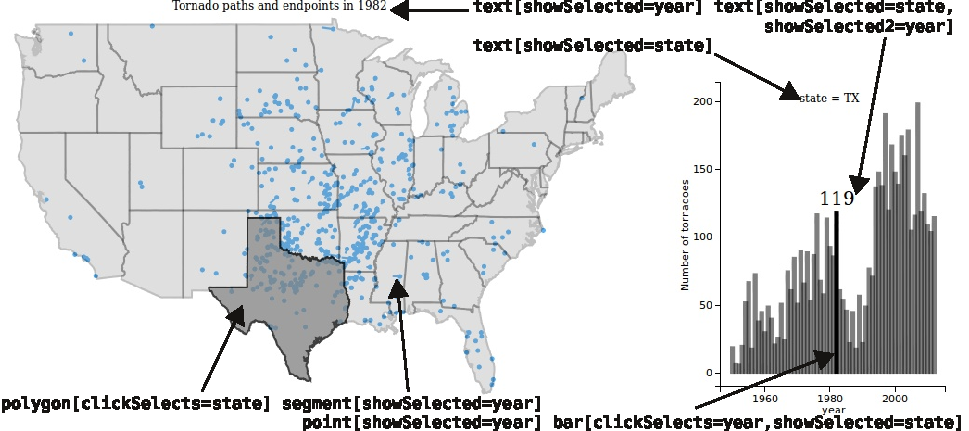
\includegraphics{images/figure-tornado}
\caption{\label{fig:tornado}Interactive animation of US tornadoes from 1950
to 2012. This diagram depicts a scenario where the user queried Texas
(by clicking the map), and the year 1982 (by clicking the bar chart). In
addition to the graphical elements being (automatically) highlighted as
a visual clue of what query is being made, this visualization includes
dynamic labels reflecting the query. Particular queries may also be
stored and shared via a URL, for example:
\url{https://bl.ocks.org/faizan-khan-iit/raw/b3912f21ec2750f96e8d1bd4b66463b2/\#year=\%7B1982\%7Dstate=\%7BTX\%7D}.
In this link to the interactive version, we also demonstrate the ability
to dynamically rescale axes when a new query is triggered. The middle
and right panel display the same data, but use different scaling: the
middle panel reflects the `global' range (US) while the right panel
reflects the `local' range (Arkansas). Futhermore, when an axis update
is triggered, it smoothly transitions from one state to next (preserving
object constancy in the axis ticks). This helps the viewer better
perceive/understand how the range has changed from one state to the
next.}
\end{figure}

\hypertarget{central-american-climate-data}{%
\subsection{Central American Climate
data}\label{central-american-climate-data}}

\begin{figure}
\centering
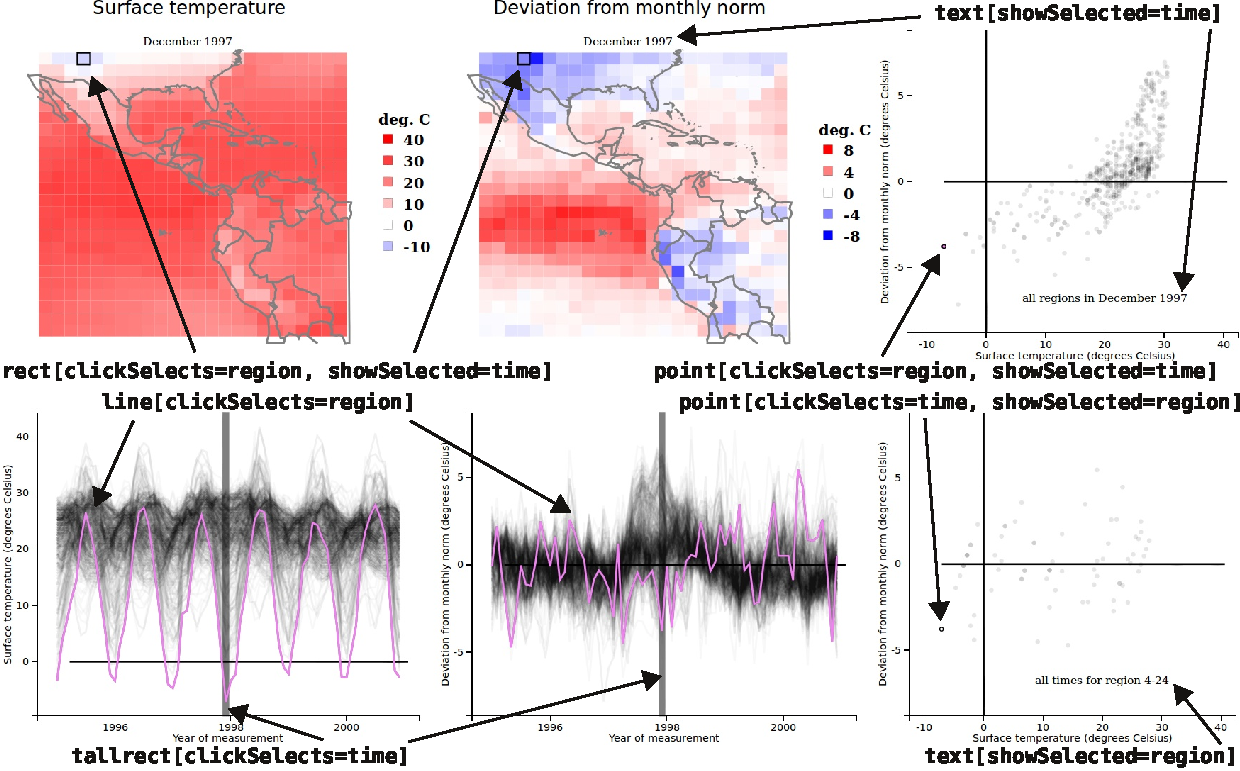
\includegraphics{images/figure-climate}
\caption{\label{fig:climate}Visualization containing 6 linked, interactive,
animated plots of Central American climate data. Top: for the selected
time (December 1997), maps displaying the spatial distribution of two
temperature variables, and a scatterplot of these two variables. The
selected region is displayed with a black outline, and can be changed by
clicking a rect on the map or a point on the scatterplot. Bottom: time
series of the two temperature variables with the selected region shown
in violet, and a scatterplot of all times for that region. The selected
time can be changed by clicking a background tallrect on a time series
or a point on the scatterplot. The selected region can be changed by
clicking a line on a time series.}
\end{figure}

Figure \ref{fig:climate} depicts an interactive animation of climate
time series data observed in Central America. Two maps display the
spatial distribution of sea surface temperature as well as its deviation
from its monthly norm. Conditioning on a particular cell/region
highlights that region's corresponding time series below the map,
allowing one to assess whether a particularly low/high value at one time
point remains so over time. Scatterplots also show the relationships
between the two temperature variables for the selected time and region,
allowing us to further examine how unusual a particular query is with
respect to both time and space.

Summary statistics describing complexity and performance of examples in
this paper, as well as other \textbf{animint} examples, are displayed in
Table \ref{tab:examples}. The climate data visualization has noticeably
slow animations, since it displays about 88,980 geometric elements at
once (\url{http://bit.ly/QcUrhn}). We observed this slowdown across all
browsers, which suggested that there is an inherent bottleneck when
rendering large interactive plots in web browsers using JavaScript and
SVG. Another \textbf{animint} with a similar amount of total rows is
based on the evolution data
(\url{http://members.cbio.ensmp.fr/~thocking/animint/evolution/viz.html}),
but since it shows less data onscreen (about 2,703 elements), it
exhibits faster responses to interactivity and animation.

\textbf{animint} is still useful for creating interactive but
non-animated plots when there is not a time variable in the data. In
fact, 7 of the 11 examples in Table \ref{tab:examples} are not animated.
For example, linked plots are useful to illustrate complex concepts such
as a change point detection model in the breakpoints data
(\url{http://members.cbio.ensmp.fr/~thocking/animint/breakpoints/viz.html}).
The user can explore different model parameters and data sets since
these are encoded as \textbf{animint} interaction variables.

\begin{table}

\caption{
Characteristics of 11 interactive visualizations designed with
    \textbf{animint}. The interactive version of these visualizations can be accessed 
    via \url{http://members.cbio.ensmp.fr/~thocking/animint/}.
    From left to right, we show the data set name and 
    Figure number in this paper (Figure), the
    lines of R code (LOC) including data processing but not including comments
    (80 characters max per line),
    the amount of time it takes to compile the visualization (seconds),
    the total size of the uncompressed TSV files in megabytes (MB),
    the total number of data points (rows),
    the median number of data points shown at once (onscreen),
    the number of data columns visualized (vars),
    the number of \texttt{clickSelects}/\texttt{showSelected} 
    variables (int),
    the number of linked panels (plots),
    if the plot is animated.
}\label{tab:examples}

\begin{tabularx}{\textwidth}{|l|l|l|l|l|l|l|l|l|l|l|}
    \hline
 Figure & LOC & seconds & MB & rows & onscreen & vars & int & plots & animated? \\ 
  \hline
  worldPop & 17 & 0.2 & 0.1 & 924 & 624 &  4 &  2 &  2 & yes  \\ 
  WorldBank \ref{fig:worldbank} & 20 & 2.3 & 2.1 & 34132 & 11611 &  6 &  2 &  2 & yes \\ 
  evolution & 25 & 21.6 & 12.0 & 240600 & 2703 &  5 &  2 &  2 & yes  \\ 
  change & 36 & 2.8 & 2.5 & 36238 & 25607 & 12 &  2 &  3 & no  \\ 
  tornado  \ref{fig:tornado} & 39 & 1.7 & 6.1 & 103691 & 16642 & 11 &  2 &  2 & no \\ 
  prior & 54 & 0.7 & 0.2 & 1960 & 142 & 12 &  3 &  4 & no  \\ 
  compare & 66 & 10.7 & 7.9 & 133958 & 2140 & 20 &  2 &  5 & no  \\ 
  breakpoints & 68 & 0.5 & 0.3 & 4242 & 667 & 13 &  2 &  3 & no  \\ 
  climate \ref{fig:climate} & 84 & 12.8 & 19.7 & 253856 & 88980 & 15 &  2 &  6 & yes \\ 
  scaffolds & 110 & 56.3 & 78.5 & 618740 & 9051 & 30 &  3 &  3 & no  \\ 
  ChIPseq & 229 & 29.9 & 78.3 & 1292464 & 1156 & 44 &  4 &  5 & no  \\
  \hline
\end{tabularx}

\end{table}

\hypertarget{compare}{%
\section{Comparison study}\label{compare}}

In this section we compare our \textbf{animint} implementation with
other similar leading systems by creating a given visualization in each
system and discussing the pros and cons of the different approaches.

\hypertarget{tour}{%
\subsection{The Grand Tour}\label{tour}}

The Grand Tour is a well-known method for viewing high dimensional data
which requires interactive and dynamic graphics (Asimov 1985). Figure
\ref{fig:tour} shows a grand tour of 300 observations sampled from a
correlated tri-variate normal distribution. The left hand view shows the
marginal density of each point while the right hand view ``tours''
through 2D projections of the 3D data. There are many ways to choose
projections in a tour, and many ways to interpolate between projections,
most of which can be programmed fairly easily using R and relevant
add-on packages. In this case, we used the R package \textbf{tourr},
which uses the geodesic random walk (i.e., random 2D projection with
geodesic interpolation) in its grand tour algorithm (Wickham et al.
2011).

\begin{figure}
\centering
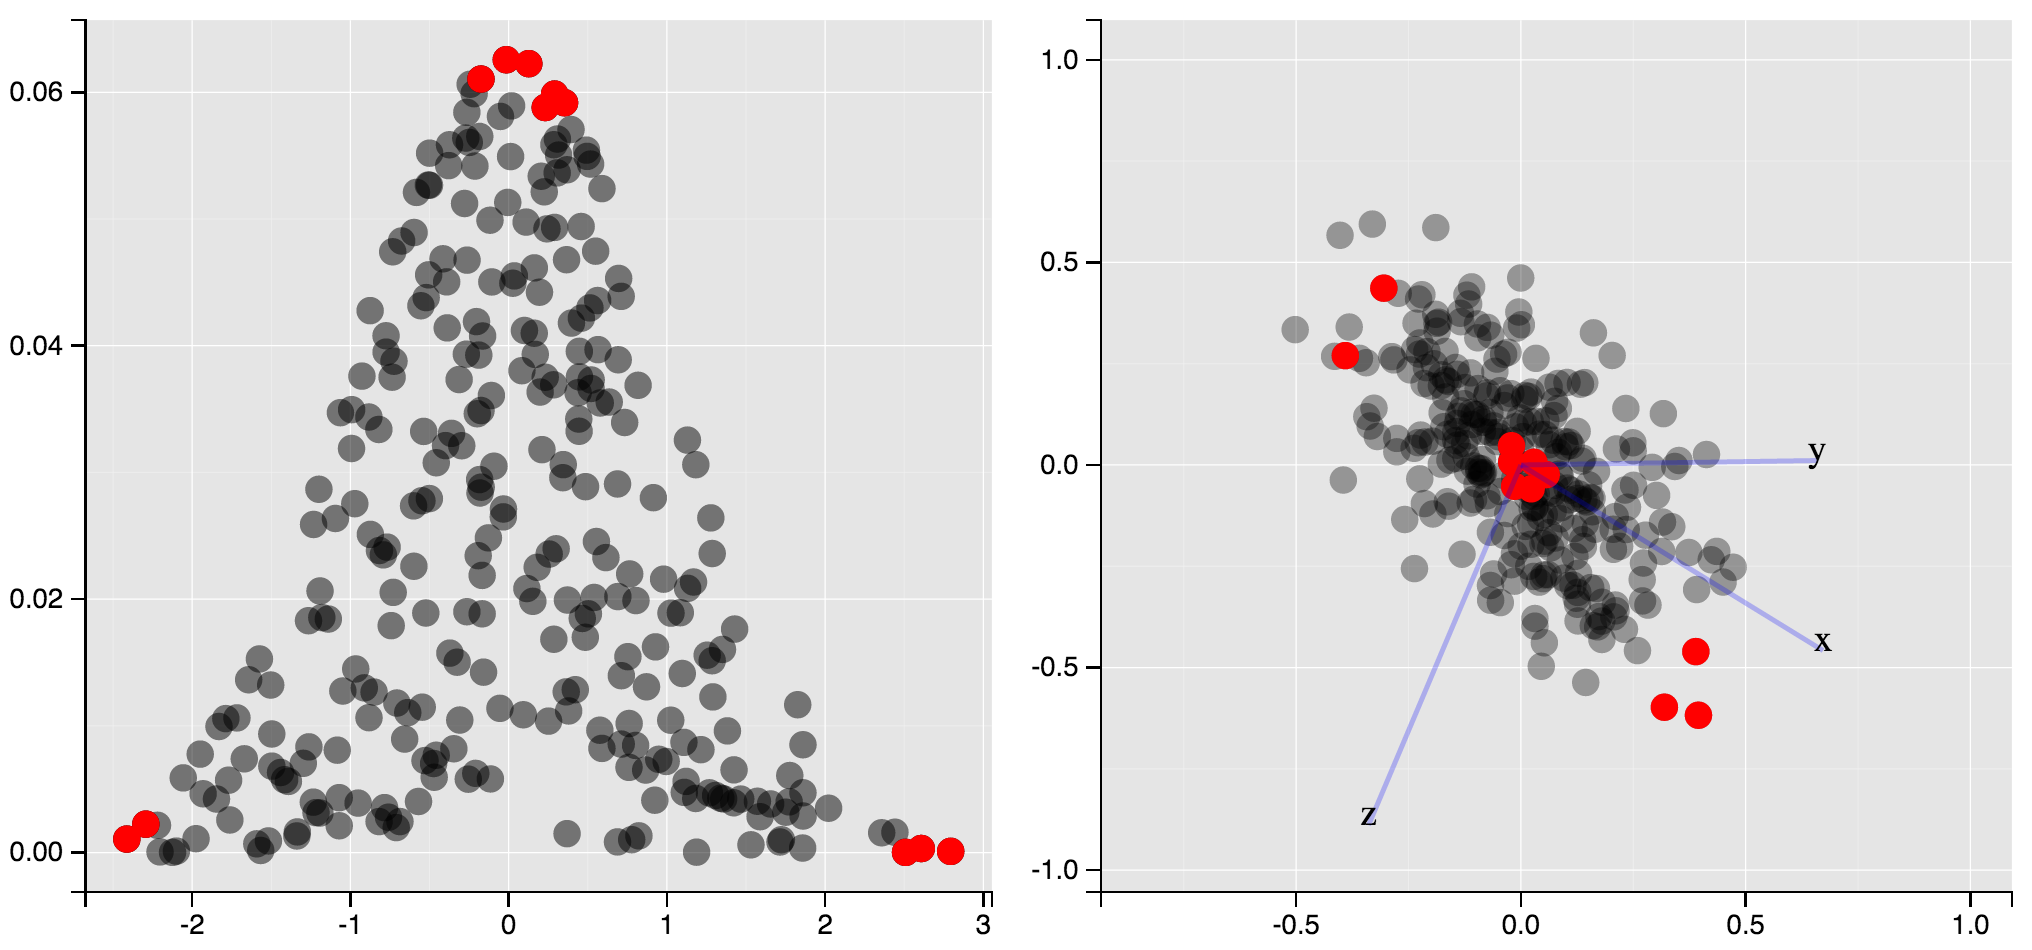
\includegraphics{images/tour}
\caption{\label{fig:tour}Linked selection in a grand tour with
\textbf{animint}. A video demonstration can be viewed online at
\url{https://vimeo.com/160720834}}
\end{figure}

When touring data, it is generally useful to link low-dimensional
displays with the tour itself. The video in Figure \ref{fig:tour} was
generated with our current \textbf{animint} implementation, and points
are selected via mouse click which reveals that points with high
marginal density are located in the ellipsoid center while points with a
low marginal density appear near the ellipsoid border. In this case, it
would be convenient to also have brush selection, as we demonstrate in
Figure \ref{fig:tourbrush} which implements the same touring example
using the R packages \textbf{ggvis} and \textbf{shiny}. The brush in
Figure \ref{fig:tourbrush} is implemented with \textbf{shiny}'s support
for brushing static images, which currently does not support multiple
brushes, making it difficult to select non-contiguous regions.

\begin{figure}
\centering
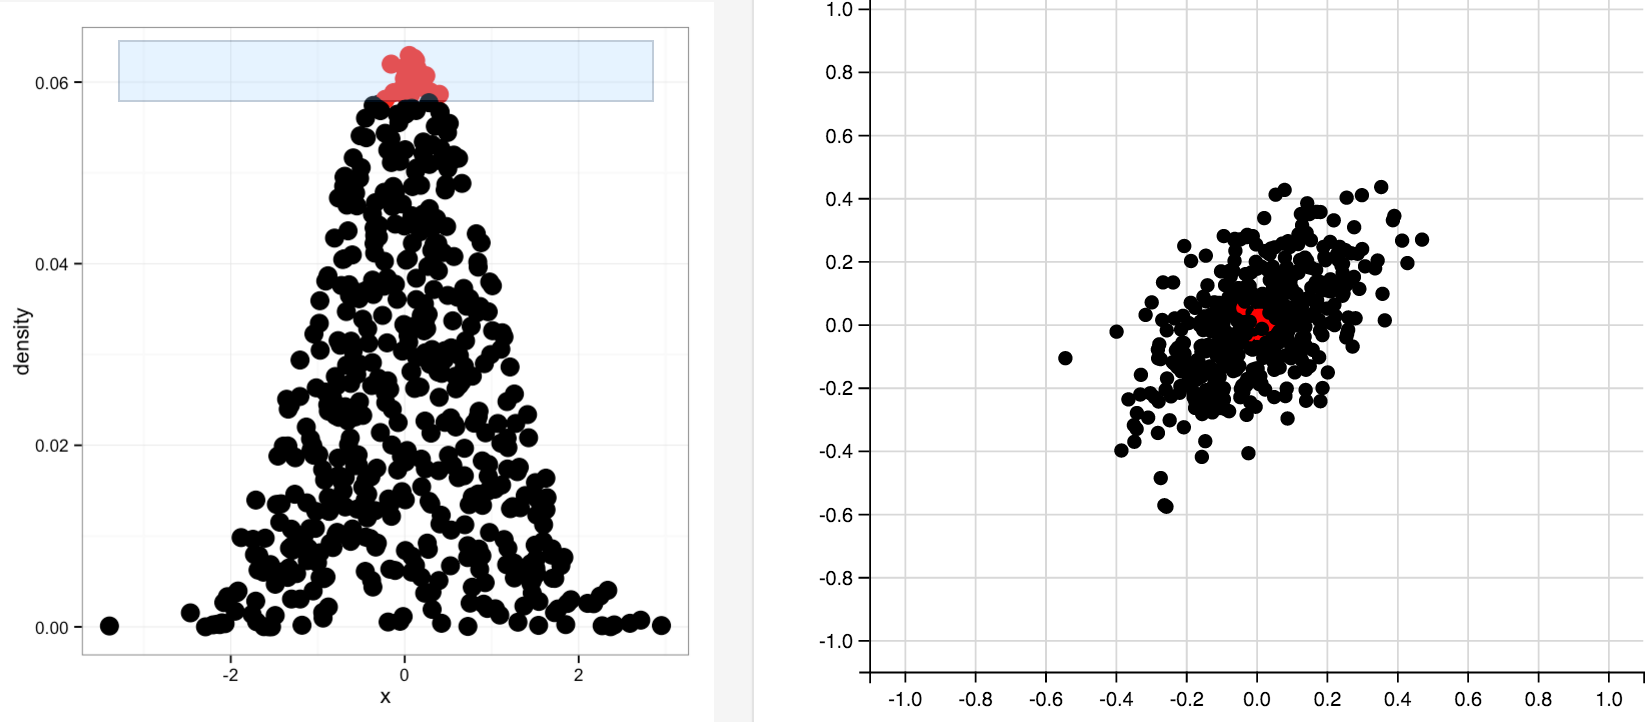
\includegraphics{images/tourbrush}
\caption{\label{fig:tourbrush}Linked selection in a grand tour with
\textbf{ggvis} and \textbf{shiny}. A video demonstration can be viewed
online at \url{https://vimeo.com/160825528}}
\end{figure}

This example helps point out a few other important differences in using
\textbf{animint} versus \textbf{ggvis}+\textbf{shiny} to implement
``multiple linked and dynamic views'' as described in Ahlberg,
Williamson, and Shneiderman (1991) and Buja et al. (1991). Maintaining
state of the linked brush in Figure \ref{fig:tourbrush} requires both
knowledge and clever use of some sophicated programming techniques such
as closures and reactivity. It also requires knowledge of the
\textbf{shiny} web application framework and a new approach to the
grammar of graphics. On the other hand, maintaining state in Figure
\ref{fig:tour} requires a few different
\texttt{clickSelects}/\texttt{showSelected} mappings. As a result, we
believe \textbf{animint} provides a more elegant user interface for this
application.

The touring example also helps point out important consequences of the
design and implementation of these two different systems. As mentioned
in Section \ref{implementation}, our current \textbf{animint}
implementation requires every subset of data to be precomputed before
render time. For visualizations such as tours, where it is more
efficient to perform statistical computations on-the-fly, this can be a
harsh restriction, but this is a restriction of our current
implementation (not a restriction of the framework itself). As a result,
when touring a large high-dimensional space, where many projections are
needed, \textbf{ggvis}+\textbf{shiny} may be desirable since the
projections are computed on the server and sent to the browser in
real-time. This works fine when the application is running and viewed on
the same host machine, but viewing such an application hosted on a
remote machine can produce staggered animations since client-server
requests must be performed, processed, and rendered roughly 30 times a
second. Also, generally speaking, the \textbf{animint} system results a
more pleasant experience when it comes to hosting and sharing
applications since it doesn't require a Web Server with R and special
software already installed.

\hypertarget{world-bank-example}{%
\subsection{World Bank example}\label{world-bank-example}}

We also recreated Figure \ref{fig:worldbank} using
\textbf{ggvis}+\textbf{shiny} (see \url{http://bit.ly/1SsJKlN}) and
Tableau (see \url{http://bit.ly/worldBank-tableau}). Even as experienced
\textbf{ggvis}+\textbf{shiny} users, we found it quite difficult to
replicate this example, and were not able to completely replicate it due
to a lack of a mechanism for coordinating indirect and direct
manipulations. Overall the visualization is pretty similar, but lacks a
few important features. In particular, there is no way to control the
selected year using both the slider (indirect) and clicking on the ggvis
plot (direct). It also lacks the ability to click on a country time
series and label the corresponding point on the scatterplot. This might
be possible, but we could not find a way to update a plot based on a
click event on a different plot. Even with this lack of functionality,
the \textbf{ggvis}+\textbf{shiny} is significantly more complicated and
requires more code (about 100 lines of code compared to 30).

It was also impossible to completely replicate Figure
\ref{fig:worldbank} using Tableau essentially because the example
requires a \emph{layered} approach to the grammar of graphics. In
particular, since graphical marks and interaction source/target(s) must
derive from the same table in Tableau, it was impossible to control the
clickable multiple time series and the clickable tallrects in different
ways based on the two different selection variables. In other words, in
Tableau, selections are managed on the plot level, but in
\textbf{animint}, selections are specific to each graphical layer.

\hypertarget{limitations}{%
\section{Limitations and future work}\label{limitations}}

The system we have proposed provides linked interactive plots via the
new \texttt{showSelected} and \texttt{clickSelects} aesthetics. The
linking between plots is rather flexible, but is limited to interactions
which are specified by the plot designer at compile-time. Our current
implementation provides a visual indication of the current selection via
semi-transparency of \texttt{clickSelects} geoms. In future work we
would like to explore more obvious visual cues that can be used to
quickly show the user the links between plots and possible interactions.

A number of limitations in our current implementation derive from the
fact that some plot features are computed once during the compilation
step, and remain static on a rendered plot. For example, users are
unable to change variable mappings after compilation. Also, when
different data subsets have very different ranges of values, it may be
preferable to recompute scales when \texttt{clickSelects} selection(s)
change. Some of these limitations can be resolved by adding interactive
widgets to ``recompile'' components hard-coded in the plot meta
information. In fact, \textbf{animint} makes it easy to embed
visualizations inside of \textbf{shiny} web applications, and we have an
example of interactively redefining variable mappings
(\url{http://bit.ly/animint-shiny}).

Our compiler also currently takes advantage of \textbf{ggplot2}
internals to compute statistics and positional adjustments before
rendering. As a result, statistics/positions will not dynamically
recompute based on selections. In other words, using
\texttt{clickSelects}/\texttt{showSelected} with non-identity
statistic(s)/position(s) may not generate a sensible result. It would be
possible, but a significant amount of work, to transfer these
computations from the compiler to the renderer.

Another set of limitations derive from our current restriction that all
subsets (corresponding to each possible selection) must be precomputed
before render time. As elucidated in Section \ref{tour}, if there is a
large space of possible selections, it is impractical to precompute
every subset before viewing. Therefore, for future work it would be
useful if the renderer could dynamically compute subsets when new
selections are made.

Our implementation is also limited to two specific types of direct
manipulation: selecting graphical elements via mouse click
(\texttt{clickSelects}), and showing/hiding related elements
(\texttt{showSelected}). However, the framework described in Section
\ref{extension} is not restricted to a particular event type, so
\texttt{hoverSelects} and \texttt{brushSelects} aesthetics could be
added, for instance. There are other types of interaction that could be
added, that wouldn't require additional extensions to the grammar of
graphics, such as: zooming, panning, and plot resizing.

\hypertarget{conclusion}{%
\section{Conclusion}\label{conclusion}}

We have proposed several extensions to \textbf{ggplot2}'s layered
grammar of graphics in order to support a declarative approach to
producing interactive and dynamic web graphics. By adding clickSelects
and showSelected aesthetics to specify selection source(s) and
target(s), \textbf{ggplot2} users can quickly and easily create
animations with smooth transitions and perform dynamic queries via
direct manipulation of linked views. As a result, \textbf{animint} is a
useful tool not only for EDA, but also for the presentation and
distribution of interactive statistical graphics.

\section*{Acknowledgements}

The authors wish to thank \textbf{animint} users MC Du Plessis, Song
Liu, Nikoleta Juretic, and Eric Audemard who have contributed
constructive criticism and helped its development.

\section*{References}

\hypertarget{refs}{}
\leavevmode\hypertarget{ref-Ahlberg:1991}{}%
Ahlberg, Christopher, Christopher Williamson, and Ben Shneiderman. 1991.
``Dynamic Queries for Information Exploration: An Implementation and
Evaluation.'' In \emph{ACM Chi '92 Conference Proceedings}, 21:619--26.

\leavevmode\hypertarget{ref-viewing-pipeline}{}%
Andreas Buja, Catherine Hurley, Daniel Asimov, and John A. McDonald.
1988. ``Elements of a Viewing Pipeline for Data Analysis.'' In
\emph{Dynamic Graphics for Statistics}, edited by William S. Cleveland
and Marylyn E. McGill. Belmont, California: Wadsworth, Inc.

\leavevmode\hypertarget{ref-grand-tour}{}%
Asimov, Daniel. 1985. ``The Grand Tour: A Tool for Viewing
Multidimensional Data.'' \emph{SIAM J. Sci. Stat. Comput.} 6 (1).
Philadelphia, PA, USA: Society for Industrial; Applied
Mathematics:128--43. \url{https://doi.org/10.1137/0906011}.

\leavevmode\hypertarget{ref-brushing-scatterplots}{}%
Becker, RA, and WS Cleveland. 1987. ``Brushing Scatterplots.''
\emph{Technometrics} 29 (2):127--42.

\leavevmode\hypertarget{ref-trellis}{}%
Becker, Richard A., William S. Cleveland, and Ming-Jen Shyu. 2010. ``The
Visual Design and Control of Trellis Displays.'' \emph{Journal of
Computational and Graphical Statistics} 19 (1). Taylor \& Francis:3--28.

\leavevmode\hypertarget{ref-d3}{}%
Bostock, Michael, Vadim Oglevetsky, and Jeffrey Heer. 2011. ``D3
Data-Driven Documents.'' \emph{IEEE Transactions on Visualization and
Computer Graphics} 17 (12):2301--9.

\leavevmode\hypertarget{ref-Buja:1991vh}{}%
Buja, Andreas, John Alan McDonald, John Michalak, and Werner Stuetzle.
1991. ``Interactive data visualization using focusing and linking.''
\emph{IEEE Proceedings of Visualization}, February, 1--8.

\leavevmode\hypertarget{ref-cairo}{}%
Cairo. 2016. ``Cairo: A Vector Graphics Library.''
\url{http://cairographics.org/}.

\leavevmode\hypertarget{ref-ggvis}{}%
Chang, Winston, and Hadley Wickham. 2015. \emph{ggvis: Interactive
Grammar of Graphics}. \url{https://CRAN.R-project.org/package=ggvis}.

\leavevmode\hypertarget{ref-Cook:2007uk}{}%
Cook, Dianne, Andreas Buja, and Deborah F Swayne. 2007. ``Interactive
High-Dimensional Data Visualization.'' \emph{Journal of Computational
and Graphical Statistics}, December, 1--23.

\leavevmode\hypertarget{ref-ggobi:2007}{}%
Cook, Dianne, and Deborah F. Swayne. 2007. \emph{Interactive and Dynamic
Graphics for Data Analysis : With R and Ggobi}. Use R ! New York:
Springer. \url{http://www.ggobi.org/book/}.

\leavevmode\hypertarget{ref-Donoho:2015tu}{}%
Donoho, David. 2015. ``50 years of Data Science.''
\url{https://dl.dropboxusercontent.com/u/23421017/50YearsDataScience.pdf}.

\leavevmode\hypertarget{ref-rggobi}{}%
Duncan Temple Lang, Hadley Wickham, Debby Swayne. 2016. \emph{Interface
Between R and 'Ggobi'}.

\leavevmode\hypertarget{ref-PRIM9}{}%
Fisherkeller, Friedman, M. A., and J. W. Tukey. 1988. ``PRIM-9, an
Interactive Multidimensional Data Display and Analysis System.'' In
\emph{Dynamic Graphics for Statistics}, 91--109.

\leavevmode\hypertarget{ref-qtbase}{}%
Lawrence, Michael, and Deepayan Sarkar. 2016. \emph{Interface Between R
and Qt}. \url{https://github.com/ggobi/qtbase}.

\leavevmode\hypertarget{ref-RGtk2}{}%
Lawrence, Michael, and Duncan Temple Lang. 2010. ``RGtk2: A Graphical
User Interface Toolkit for R.'' \emph{Journal of Statistical Software}
37 (8):1--52. \url{http://www.jstatsoft.org/v37/i08/}.

\leavevmode\hypertarget{ref-gridSVG}{}%
Murrell, Paul, and Simon Potter. 2015. \emph{GridSVG: Export 'Grid'
Graphics as Svg}. \url{https://CRAN.R-project.org/package=gridSVG}.

\leavevmode\hypertarget{ref-SVGAnnotation}{}%
Nolan, Deborah, and Duncan Temple Lang. 2012. ``Interactive and Animated
Scalable Vector Graphics and R Data Displays.'' \emph{Journal of
Statistical Software} 46 (1):1--88.
\url{http://www.jstatsoft.org/v46/i01/}.

\leavevmode\hypertarget{ref-opencpu}{}%
Ooms, Jeroen. 2014. ``The Opencpu System: Towards a Universal Interface
for Scientific Computing Through Separation of Concerns.''
\emph{arXiv:1406.4806 {[}stat.CO{]}}.
\url{http://arxiv.org/abs/1406.4806}.

\leavevmode\hypertarget{ref-RCore}{}%
R Core Team. 2017. \emph{R: A Language and Environment for Statistical
Computing}. Vienna, Austria: R Foundation for Statistical Computing.
\url{http://www.R-project.org/}.

\leavevmode\hypertarget{ref-gganimate}{}%
Robinson, David. 2016. \emph{gganimate: Create easy animations with
ggplot2}. \url{http://github.com/dgrtwo/gganimate}.

\leavevmode\hypertarget{ref-shiny}{}%
RStudio. 2013. ``Shiny: Easy Web Applications in R.''
\url{http://www.rstudio.com/shiny/}.

\leavevmode\hypertarget{ref-xgobi}{}%
Swayne, Cook, D. F., and A. Buja. 1998. ``XGobi: Interactive Dynamic
Data Visualization in the X Window System.'' \emph{Journal of
Computational and Graphical Statistics} 7 (1):113--30.

\leavevmode\hypertarget{ref-mondrian}{}%
Theus, M. 2002. ``Interactive Data Visualization Using Mondrian.''
\emph{Journal of Statistical Software} 7 (11):1--9.
\url{http://www.jstatsoft.org/v07/i11}.

\leavevmode\hypertarget{ref-LISP-STAT}{}%
Tierney, Luke. 1990. \emph{LISP-Stat: An Object Oriented Environment for
Statistical Computing and Dynamic Graphics.} Wiley-Interscience, New
York.

\leavevmode\hypertarget{ref-plumber}{}%
Trestle Technology, LLC. 2017. \emph{Plumber: An Api Generator for R}.
\url{https://CRAN.R-project.org/package=plumber}.

\leavevmode\hypertarget{ref-vega}{}%
Trifacta. 2014. ``Vega: A Declarative Visualization Grammar.''
\url{http://trifacta.github.io/vega/}.

\leavevmode\hypertarget{ref-MANET}{}%
Unwin A., Hofmann H., Hawkins G. 1996. ``Interactive Graphics for Data
Sets with Missing Values - Manet.'' \emph{Journal of Computational and
Graphical Statistics} 4 (6).

\leavevmode\hypertarget{ref-Urbanek2011}{}%
Urbanek, Simon. 2011. ``IPlots eXtreme: Next-Generation Interactive
Graphics Design and Implementation of Modern Interactive Graphics.''
\emph{Computational Statistics} 26 (3):381--93.
\url{https://doi.org/10.1007/s00180-011-0240-x}.

\leavevmode\hypertarget{ref-rJava}{}%
---------. 2016. \emph{RJava: Low-Level R to Java Interface}.
\url{https://CRAN.R-project.org/package=rJava}.

\leavevmode\hypertarget{ref-FastRWeb}{}%
Urbanek, Simon, and Jeffrey Horner. 2015. \emph{FastRWeb: Fast
Interactive Framework for Web Scripting Using R}.
\url{https://CRAN.R-project.org/package=FastRWeb}.

\leavevmode\hypertarget{ref-loon}{}%
Waddell, Adrian, and R. Wayne Oldford. 2018. \emph{Loon: Interactive
Statistical Data Visualization}.
\url{https://CRAN.R-project.org/package=loon}.

\leavevmode\hypertarget{ref-ggplot2-book}{}%
Wickham, Hadley. 2009. \emph{ggplot2: elegant graphics for data
analysis}. Springer New York. \url{http://had.co.nz/ggplot2/book}.

\leavevmode\hypertarget{ref-tourr}{}%
Wickham, Hadley, Dianne Cook, Heike Hofmann, and Andreas Buja. 2011.
``tourr: An R Package for Exploring Multivariate Data with
Projections,'' April, 1--18.

\leavevmode\hypertarget{ref-plumbing}{}%
Wickham, Hadley, Michael Lawrence, Dianne Cook, Andreas Buja, Heike
Hofmann, and Deborah F Swayne. 2010. ``The Plumbing of Interactive
Graphics.'' \emph{Computational Statistics}, April, 1--7.

\leavevmode\hypertarget{ref-wilkinson}{}%
Wilkinson, Leland, D Wills, D Rope, A Norton, and R Dubbs. 2006.
\emph{The Grammar of Graphics}. Springer.

\leavevmode\hypertarget{ref-WorldBank}{}%
World Bank. 2012. ``World Development Indicators.''
\url{http://data.worldbank.org/data-catalog/world-development-indicators}.

\leavevmode\hypertarget{ref-animation}{}%
Xie, Yihui. 2013. ``animation: An R Package for Creating Animations and
Demonstrating Statistical Methods.'' \emph{Journal of Statistical
Software} 53 (1):1--27. \url{http://www.jstatsoft.org/v53/i01/}.

\leavevmode\hypertarget{ref-cranvas}{}%
Xie, Yihui, Heike Hofmann, Di Cook, Xiaoyue Cheng, Barret Schloerke,
Marie Vendettuoli, Tengfei Yin, Hadley Wickham, and Michael Lawrence.
2013. \emph{Interactive Statistical Graphics Based on Qt}.



\end{document}
